\setAuthor{Richard Luhtaru}
\setRound{lõppvoor}
\setYear{2022}
\setNumber{G 3}
\setDifficulty{3}
\setTopic{TODO}

\prob{Silinder}
\begin{wrapfigure}{r}{5cm}
  \vspace{-2em}
  \begin{center}
    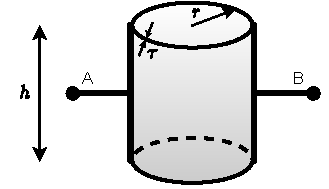
\includegraphics[width=\linewidth]{2022-v3g-03-yl.pdf}
  \end{center}
  \vspace{-2em}
\end{wrapfigure}

Õhukese silindri eritakistus on $\rho$, raadius on $r$, kõrgus on $h$ ja paksus on $\tau$. Silindri ringikujulised põhjad on eemaldatud ning silindri vastaspooltel on silindri materjal asendatud peenikeste juhtivate klemmidega, mille pikkus on $h$ ja paksus on $\tau$ (A ja B joonisel). Leidke kahe klemmi vaheline takistus.



\hint

\solu
\
Jagame silindri kaheks poolsilindriks. Me võime vaadelda kumbagi poolsilindrit kui hästi laia juhet, mille pikkus on $\ell = \pi r$ ja ristlõikepindala on $S = \tau h$. Kummagi poolsilindri takistus on seega
\begin{equation*}
    R = \rho \frac{\ell}{S} = \frac{\rho \pi r}{\tau h}
\end{equation*}

Kuna kaks ``juhet'' on ühendatud rööbiti, siis kogutakistus A ja B vahel on
\begin{equation*}
    R_{AB} = \frac{1}{2}R = \frac{\rho \pi r}{2\tau h}
\end{equation*}
\probend